\documentclass[twoside]{book}

% Packages required by doxygen
\usepackage{fixltx2e}
\usepackage{calc}
\usepackage{doxygen}
\usepackage[export]{adjustbox} % also loads graphicx
\usepackage{graphicx}
\usepackage[utf8]{inputenc}
\usepackage{makeidx}
\usepackage{multicol}
\usepackage{multirow}
\PassOptionsToPackage{warn}{textcomp}
\usepackage{textcomp}
\usepackage[nointegrals]{wasysym}
\usepackage[table]{xcolor}

% NLS support packages
\usepackage[spanish]{babel}
% Font selection
\usepackage[T1]{fontenc}
\usepackage[scaled=.90]{helvet}
\usepackage{courier}
\usepackage{amssymb}
\usepackage{sectsty}
\renewcommand{\familydefault}{\sfdefault}
\allsectionsfont{%
  \fontseries{bc}\selectfont%
  \color{darkgray}%
}
\renewcommand{\DoxyLabelFont}{%
  \fontseries{bc}\selectfont%
  \color{darkgray}%
}
\newcommand{\+}{\discretionary{\mbox{\scriptsize$\hookleftarrow$}}{}{}}

% Page & text layout
\usepackage{geometry}
\geometry{%
  a4paper,%
  top=2.5cm,%
  bottom=2.5cm,%
  left=2.5cm,%
  right=2.5cm%
}
\tolerance=750
\hfuzz=15pt
\hbadness=750
\setlength{\emergencystretch}{15pt}
\setlength{\parindent}{0cm}
\setlength{\parskip}{3ex plus 2ex minus 2ex}
\makeatletter
\renewcommand{\paragraph}{%
  \@startsection{paragraph}{4}{0ex}{-1.0ex}{1.0ex}{%
    \normalfont\normalsize\bfseries\SS@parafont%
  }%
}
\renewcommand{\subparagraph}{%
  \@startsection{subparagraph}{5}{0ex}{-1.0ex}{1.0ex}{%
    \normalfont\normalsize\bfseries\SS@subparafont%
  }%
}
\makeatother

% Headers & footers
\usepackage{fancyhdr}
\pagestyle{fancyplain}
\fancyhead[LE]{\fancyplain{}{\bfseries\thepage}}
\fancyhead[CE]{\fancyplain{}{}}
\fancyhead[RE]{\fancyplain{}{\bfseries\leftmark}}
\fancyhead[LO]{\fancyplain{}{\bfseries\rightmark}}
\fancyhead[CO]{\fancyplain{}{}}
\fancyhead[RO]{\fancyplain{}{\bfseries\thepage}}
\fancyfoot[LE]{\fancyplain{}{}}
\fancyfoot[CE]{\fancyplain{}{}}
\fancyfoot[RE]{\fancyplain{}{\bfseries\scriptsize Generado por Doxygen }}
\fancyfoot[LO]{\fancyplain{}{\bfseries\scriptsize Generado por Doxygen }}
\fancyfoot[CO]{\fancyplain{}{}}
\fancyfoot[RO]{\fancyplain{}{}}
\renewcommand{\footrulewidth}{0.4pt}
\renewcommand{\chaptermark}[1]{%
  \markboth{#1}{}%
}
\renewcommand{\sectionmark}[1]{%
  \markright{\thesection\ #1}%
}

% Indices & bibliography
\usepackage{natbib}
\usepackage[titles]{tocloft}
\setcounter{tocdepth}{3}
\setcounter{secnumdepth}{5}
\makeindex

% Hyperlinks (required, but should be loaded last)
\usepackage{ifpdf}
\ifpdf
  \usepackage[pdftex,pagebackref=true]{hyperref}
\else
  \usepackage[ps2pdf,pagebackref=true]{hyperref}
\fi
\hypersetup{%
  colorlinks=true,%
  linkcolor=blue,%
  citecolor=blue,%
  unicode%
}

% Custom commands
\newcommand{\clearemptydoublepage}{%
  \newpage{\pagestyle{empty}\cleardoublepage}%
}

\usepackage{caption}
\captionsetup{labelsep=space,justification=centering,font={bf},singlelinecheck=off,skip=4pt,position=top}

%===== C O N T E N T S =====

\begin{document}

% Titlepage & ToC
\hypersetup{pageanchor=false,
             bookmarksnumbered=true,
             pdfencoding=unicode
            }
\pagenumbering{roman}
\begin{titlepage}
\vspace*{7cm}
\begin{center}%
{\Large Juego de Barcos \\[1ex]\large 0.\+1 }\\
\vspace*{1cm}
{\large Generado por Doxygen 1.8.11}\\
\end{center}
\end{titlepage}
\clearemptydoublepage
\tableofcontents
\clearemptydoublepage
\pagenumbering{arabic}
\hypersetup{pageanchor=true}

%--- Begin generated contents ---
\chapter{juego\+Barcos}
\label{index}\hypertarget{index}{}El típico juego de hundir la flota en el que hay que bombardear por coordenadas 
\chapter{Análisis de Requisitos}
\label{md_doc_AnalisisRequisitos}
\hypertarget{md_doc_AnalisisRequisitos}{}
\subsection*{Requisitos Funcionales}


\begin{DoxyItemize}
\item R\+F1\+: Juego por turnos para 2 jugadores en red
\item R\+F2\+: Existe un tablero de 10x10 para cada jugador. Cada posición del tablero estará representada por coordenadas\+:
\begin{DoxyItemize}
\item Horizontal\+: letras mayúsculas de izquierda a derecha
\item Vertical\+: números en sentido descendente
\end{DoxyItemize}
\item R\+F3\+: Cada jugador posicionara 5 barcos en horizontal o vertical dentro de su tablero y sin que se solapen. Esta posición se mantendrá hasta el final de la partida.
\item R\+F4\+: El jugador que tiene el turno enviara unas coordenadas (p.\+e. \+: A-\/3). El programa remoto responderá\+:
\begin{DoxyItemize}
\item Agua, si en esa coordenada no tiene
\item Tocado
\item Tocado y hundido
\end{DoxyItemize}
\item R\+F5\+: El programa tendrá una interfaz de configuración con las siguientes características\+:
\begin{DoxyItemize}
\item Se deberá mostrar el tablero vacío a la izquierda con las coordenadas visibles.
\item Se deberán mostrar los barcos que hay que colocar a la derecha del tablero.
\item Deberá permitir ir introduciendo los barcos y se actualizará cada vez que introduzcamos un barco.
\end{DoxyItemize}
\item R\+F6\+: La introducción de barcos seguirá las siguientes reglas\+:
\begin{DoxyItemize}
\item Los barcos deberán situarse dentro de los límites del tablero.
\item No podrán situarse barcos en casillas contiguas.
\end{DoxyItemize}
\item R\+F7\+: La interfaz de juego deberá cumplir\+:
\begin{DoxyItemize}
\item Mostrar el tablero propio con los barcos colocados a la izquierda.
\item Mostrar el tablero enemigo con las casillas reveladas a la derecha.
\item Cualquier movimiento enemigo deberá ser actualizado en el tablero propio.
\item Cualquier movimiento propio deberá ser actualizado en el tablero enemigo.
\end{DoxyItemize}
\item R\+F8\+: Normas del juego.
\begin{DoxyItemize}
\item Una vez posicionados los barcos de acuerdo a las reglas iniciará el juego el primer jugador que haya terminado de definir los barcos.
\item Los jugadores introducirán unas coordenadas por turnos con los siguientes posibles resultados\+:
\begin{DoxyItemize}
\item Agua\+: El jugador no ha acertado la posición de un barco enemigo.
\item Tocado\+: El jugador ha acertado la posición de un barco enemigo.
\item Tocado y Hundido\+: El jugador ha acertado la posición de un barco enemigo y lo ha destruido.
\end{DoxyItemize}
\item Cuando un jugador consiga un Tocado o un Tocado y Hundido podrá volver a jugar su turno.
\item El juego finaliza cuando un jugador ha Tocado y Hundido todos los barcos enemigos. 
\end{DoxyItemize}
\end{DoxyItemize}
\chapter{Indice de archivos}
\section{Lista de archivos}
Lista de todos los archivos documentados y con descripciones breves\+:\begin{DoxyCompactList}
\item\contentsline{section}{\hyperlink{main_8c}{main.\+c} }{\pageref{main_8c}}{}
\item\contentsline{section}{src/{\bfseries tablero.\+c} }{\pageref{tablero_8c}}{}
\item\contentsline{section}{src/\hyperlink{tablero_8h}{tablero.\+h} \\*Librería de tablero }{\pageref{tablero_8h}}{}
\end{DoxyCompactList}

\chapter{Documentación de archivos}
\hypertarget{main_8c}{}\section{Referencia del Archivo main.\+c}
\label{main_8c}\index{main.\+c@{main.\+c}}
{\ttfamily \#include \char`\"{}src/tablero.\+h\char`\"{}}\\*
Dependencia gráfica adjunta para main.\+c\+:\nopagebreak
\begin{figure}[H]
\begin{center}
\leavevmode
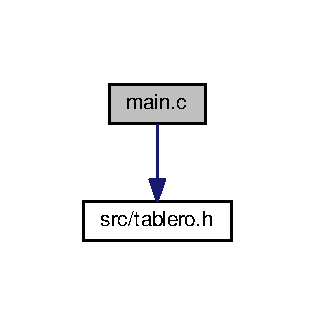
\includegraphics[width=151pt]{main_8c__incl}
\end{center}
\end{figure}
\subsection*{Funciones}
\begin{DoxyCompactItemize}
\item 
int \hyperlink{main_8c_ae66f6b31b5ad750f1fe042a706a4e3d4}{main} ()
\begin{DoxyCompactList}\small\item\em Método de prueba. \end{DoxyCompactList}\end{DoxyCompactItemize}


\subsection{Documentación de las funciones}
\index{main.\+c@{main.\+c}!main@{main}}
\index{main@{main}!main.\+c@{main.\+c}}
\subsubsection[{\texorpdfstring{main()}{main()}}]{\setlength{\rightskip}{0pt plus 5cm}int main (
\begin{DoxyParamCaption}
{}
\end{DoxyParamCaption}
)}\hypertarget{main_8c_ae66f6b31b5ad750f1fe042a706a4e3d4}{}\label{main_8c_ae66f6b31b5ad750f1fe042a706a4e3d4}


Método de prueba. 

Inicializa un tablero con agua, cambia el valor de determinadas posiciones y finalmente lo imprime 

Definición en la línea 15 del archivo main.\+c.


\hypertarget{tablero_8h}{}\section{Referencia del Archivo src/tablero.h}
\label{tablero_8h}\index{src/tablero.\+h@{src/tablero.\+h}}


Librería de tablero.  


Gráfico de los archivos que directa o indirectamente incluyen a este archivo\+:\nopagebreak
\begin{figure}[H]
\begin{center}
\leavevmode
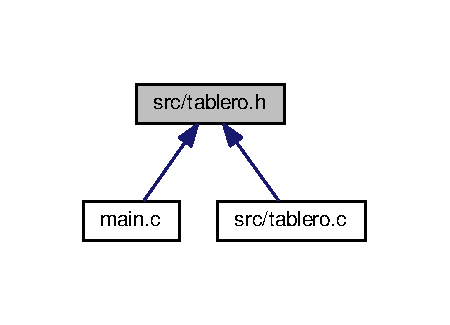
\includegraphics[width=216pt]{tablero_8h__dep__incl}
\end{center}
\end{figure}
\subsection*{\textquotesingle{}defines\textquotesingle{}}
\begin{DoxyCompactItemize}
\item 
\#define {\bfseries A\+M\+A\+R\+I\+L\+LO}~\char`\"{}\textbackslash{}033\mbox{[}1;5;3m\char`\"{}\hypertarget{tablero_8h_a706dd8cf719e6640421418eea1b08c21}{}\label{tablero_8h_a706dd8cf719e6640421418eea1b08c21}

\item 
\#define {\bfseries A\+G\+U\+A\+C\+O\+L\+OR}~\char`\"{}\textbackslash{}033\mbox{[}1;94m $\sim$\char`\"{}\hypertarget{tablero_8h_a2f9e050811f20df3bd9721fead795c90}{}\label{tablero_8h_a2f9e050811f20df3bd9721fead795c90}

\item 
\#define {\bfseries R\+E\+S\+ET}~\char`\"{}\textbackslash{}033\mbox{[}0m\char`\"{}\hypertarget{tablero_8h_ab702106cf3b3e96750b6845ded4e0299}{}\label{tablero_8h_ab702106cf3b3e96750b6845ded4e0299}

\item 
\#define {\bfseries T\+LC}~\char`\"{}┌\char`\"{}\hypertarget{tablero_8h_a0ecbf960a8f019eb82c587b6047d44f1}{}\label{tablero_8h_a0ecbf960a8f019eb82c587b6047d44f1}

\item 
\#define {\bfseries T\+RC}~\char`\"{}┐\char`\"{}\hypertarget{tablero_8h_a62d5faef958283fa41663bc9384799fd}{}\label{tablero_8h_a62d5faef958283fa41663bc9384799fd}

\item 
\#define {\bfseries HL}~\char`\"{}───\char`\"{}\hypertarget{tablero_8h_a1592226003ffbf8fa1b036eae180b6f5}{}\label{tablero_8h_a1592226003ffbf8fa1b036eae180b6f5}

\item 
\#define {\bfseries L\+CL}~\char`\"{}├\char`\"{}\hypertarget{tablero_8h_a0a81b33ee1d1f6262a7c364a027d599e}{}\label{tablero_8h_a0a81b33ee1d1f6262a7c364a027d599e}

\item 
\#define {\bfseries R\+CL}~\char`\"{}┤\char`\"{}\hypertarget{tablero_8h_a671ee4cc5791feb053a0e017c161bf04}{}\label{tablero_8h_a671ee4cc5791feb053a0e017c161bf04}

\item 
\#define {\bfseries CL}~\char`\"{}┼\char`\"{}\hypertarget{tablero_8h_a8f4ea5fa21d42f950b5f95a91e9ff227}{}\label{tablero_8h_a8f4ea5fa21d42f950b5f95a91e9ff227}

\item 
\#define {\bfseries B\+CL}~\char`\"{}┴\char`\"{}\hypertarget{tablero_8h_ad70cb678a2cc06df55b2a3d6e2a9c107}{}\label{tablero_8h_ad70cb678a2cc06df55b2a3d6e2a9c107}

\item 
\#define {\bfseries T\+CL}~\char`\"{}┬\char`\"{}\hypertarget{tablero_8h_ae7570bb64fc70bafdbbdcaae10ba9d93}{}\label{tablero_8h_ae7570bb64fc70bafdbbdcaae10ba9d93}

\item 
\#define {\bfseries VL}~\char`\"{}│\char`\"{}\hypertarget{tablero_8h_af66e7c3d47aab0745e29e697ea13c6f6}{}\label{tablero_8h_af66e7c3d47aab0745e29e697ea13c6f6}

\item 
\#define {\bfseries B\+LC}~\char`\"{}└\char`\"{}\hypertarget{tablero_8h_a2900b28f9c794085851eb8e631aaf683}{}\label{tablero_8h_a2900b28f9c794085851eb8e631aaf683}

\item 
\#define {\bfseries B\+RC}~\char`\"{}┘\char`\"{}\hypertarget{tablero_8h_a91cf1c8bed2b5667f322c71ac83e8294}{}\label{tablero_8h_a91cf1c8bed2b5667f322c71ac83e8294}

\item 
\#define {\bfseries A\+G\+UA}~\char`\"{}\textbackslash{}033\mbox{[}1;94m\textbackslash{}u2588\textbackslash{}u2588\textbackslash{}u2588\textbackslash{}033\mbox{[}0m\char`\"{}\hypertarget{tablero_8h_aac90289bb1a5731b2a955f546426c33b}{}\label{tablero_8h_aac90289bb1a5731b2a955f546426c33b}

\item 
\#define {\bfseries B\+A\+R\+CO}~\char`\"{}\textbackslash{}033\mbox{[}1;90m\textbackslash{}u2588\textbackslash{}u2588\textbackslash{}u2588\textbackslash{}033\mbox{[}0m\char`\"{}\hypertarget{tablero_8h_ad009bc87621929a3bacf62d9b0a0243b}{}\label{tablero_8h_ad009bc87621929a3bacf62d9b0a0243b}

\item 
\#define {\bfseries T\+O\+C\+A\+DO}~\char`\"{}\textbackslash{}033\mbox{[}1;93m\textbackslash{}u2588\textbackslash{}u2588\textbackslash{}u2588\textbackslash{}033\mbox{[}0m\char`\"{}\hypertarget{tablero_8h_a7eaafb90c028f39b65a302c9d1333d49}{}\label{tablero_8h_a7eaafb90c028f39b65a302c9d1333d49}

\item 
\#define {\bfseries H\+U\+N\+D\+I\+DO}~\char`\"{}\textbackslash{}033\mbox{[}1;91m\textbackslash{}u2588\textbackslash{}u2588\textbackslash{}u2588\textbackslash{}033\mbox{[}0m\char`\"{}\hypertarget{tablero_8h_a641a5e36ee010b9b82046b274458030c}{}\label{tablero_8h_a641a5e36ee010b9b82046b274458030c}

\item 
\#define {\bfseries T\+AM}~10\hypertarget{tablero_8h_ae0b4816fb45161ef9da5e6d6134ee28a}{}\label{tablero_8h_ae0b4816fb45161ef9da5e6d6134ee28a}

\end{DoxyCompactItemize}
\subsection*{Funciones}
\begin{DoxyCompactItemize}
\item 
void \hyperlink{tablero_8h_a1d9f20ce49461080e37ece95fdc19282}{inicializar\+\_\+tablero} ()
\begin{DoxyCompactList}\small\item\em Inicializa las posiciones del tablero a agua. \end{DoxyCompactList}\item 
void \hyperlink{tablero_8h_a4432f716adae12078544069edeeb8e51}{imprimir\+\_\+tablero} ()
\begin{DoxyCompactList}\small\item\em Imprimie por pantalla el estado de un tablero. \end{DoxyCompactList}\end{DoxyCompactItemize}
\subsection*{Variables}
\begin{DoxyCompactItemize}
\item 
char {\bfseries tablero} \mbox{[}T\+AM\mbox{]}\mbox{[}T\+AM\mbox{]}\hypertarget{tablero_8h_aef679ddb01db65581534a37a8b7d78ea}{}\label{tablero_8h_aef679ddb01db65581534a37a8b7d78ea}

\end{DoxyCompactItemize}


\subsection{Descripción detallada}
Librería de tablero. 

Esta librería incluye dos métodos para la inicialización y la impresión por consola del tablero

\begin{DoxyAuthor}{Autor}
Teo 
\end{DoxyAuthor}


\subsection{Documentación de las funciones}
\index{tablero.\+h@{tablero.\+h}!imprimir\+\_\+tablero@{imprimir\+\_\+tablero}}
\index{imprimir\+\_\+tablero@{imprimir\+\_\+tablero}!tablero.\+h@{tablero.\+h}}
\subsubsection[{\texorpdfstring{imprimir\+\_\+tablero()}{imprimir_tablero()}}]{\setlength{\rightskip}{0pt plus 5cm}void imprimir\+\_\+tablero (
\begin{DoxyParamCaption}
{}
\end{DoxyParamCaption}
)}\hypertarget{tablero_8h_a4432f716adae12078544069edeeb8e51}{}\label{tablero_8h_a4432f716adae12078544069edeeb8e51}


Imprimie por pantalla el estado de un tablero. 

Imprime el tablero por la consola con diferentes colores para cada estado de la casilla. 

Definición en la línea 89 del archivo tablero.\+c.

\index{tablero.\+h@{tablero.\+h}!inicializar\+\_\+tablero@{inicializar\+\_\+tablero}}
\index{inicializar\+\_\+tablero@{inicializar\+\_\+tablero}!tablero.\+h@{tablero.\+h}}
\subsubsection[{\texorpdfstring{inicializar\+\_\+tablero()}{inicializar_tablero()}}]{\setlength{\rightskip}{0pt plus 5cm}void inicializar\+\_\+tablero (
\begin{DoxyParamCaption}
{}
\end{DoxyParamCaption}
)}\hypertarget{tablero_8h_a1d9f20ce49461080e37ece95fdc19282}{}\label{tablero_8h_a1d9f20ce49461080e37ece95fdc19282}


Inicializa las posiciones del tablero a agua. 

Inicializa todas las posiciones del tablero a agua, como si estuvieran vacías 

Definición en la línea 11 del archivo tablero.\+c.


%--- End generated contents ---

% Index
\backmatter
\newpage
\phantomsection
\clearemptydoublepage
\addcontentsline{toc}{chapter}{Índice}
\printindex

\end{document}
